% !TEX TS-program = xelatex
% !TEX encoding = UTF-8
%======================================================================
%  SDR Lab -- Experiment 8: Noise figure, P1dB and IIP3 -- PRE-LAB GUIDE
%  File   : prelabs/prelab_08_nf.tex          (XeLaTeX, compile twice)
%  Layout : compact title banner, NO cover page, NO table of contents.
%
%  [INSTRUCTOR]
%   * No reference experiment was supplied for this topic; the guide follows
%     Appendix A of the regulations and the equipment table of the regulations
%     (calibrated noise source + step attenuator; two-channel signal generator
%     + power combiner).
%   * The device under test is the team's RTL-SDR at several gain settings.
%   * Pre-lab task 4 uses a READY-MADE receiver model, instructor/lab02/lab02_sim.grc,
%     which you hand out (students do not build it).  Its parameters:
%     front end NF 6 dB, IIP3 -25 dBm, 8-bit converter whose full scale equals
%     (-30 dBm - gain) at the input.  The numbers quoted from "the model" were
%     obtained by running exactly this flowgraph in GNU Radio 3.10.9.
%======================================================================
\documentclass[a4paper,11pt]{article}
\IfFileExists{../common/preamble.tex}{\def\SDRroot{..}}{\def\SDRroot{.}}
\def\SDRdoctype{prelab}
\def\SDRexpnum{2}
\def\SDRexptitle{عدد نویز و پارامترهای \lr{RF}}
\def\SDRexptitleEN{Noise Figure, P1dB and IIP3}
\input{\SDRroot/common/preamble}

\begin{document}
\SDRbanner

\begin{infostrip}
\begin{tabularx}{\linewidth}{@{}r@{\hspace{1em}}X@{}}
\textbf{مهلت تحویل} & حداکثر ۲۴ ساعت پیش از شروع جلسه، روی وب‌سایت تیم:
\code{/lab02/prelab.pdf}
و
\code{/lab02/prelab.html} \\
\textbf{زمان لازم} & حدود ۵ ساعت (برآورد)
\end{tabularx}
\end{infostrip}

%======================================================================
\isection{target}{هدف آزمایش}
%======================================================================
هر گیرنده دو مرز دارد. از پایین، نویز خودِ گیرنده تعیین می‌کند ضعیف‌ترین سیگنال قابل دریافت چقدر است؛ این مرز را \textbf{عدد نویز} می‌سنجد. از بالا، غیرخطی‌بودن تعیین می‌کند قوی‌ترین سیگنالی که گیرنده بدون خراب‌کردن آن (و بدون ساختن سیگنال‌های ناخواسته) تحمل می‌کند چقدر است؛ این مرز را \textbf{نقطهٔ تراکم یک دسی‌بل} و \textbf{نقطهٔ تقاطع مرتبهٔ سوم} می‌سنجند. فاصلهٔ این دو مرز محدودهٔ دینامیکی گیرنده است. در این آزمایش این سه کمیت را برای گیرندهٔ
\lr{SDR}
خودتان اندازه می‌گیرید و می‌بینید تنظیم بهره چگونه یکی را به بهای دیگری بهتر می‌کند.

\noindent
پس از انجام کامل این آزمایش باید بتوانید:
\begin{objectives}
\item عدد نویز و دمای نویز را تعریف کنید و عدد نویز یک زنجیره را با رابطهٔ فریس حساب کنید.
\item روش
\lr{Y-Factor}
را شرح دهید، رابطهٔ آن را به دست آورید و با آن عدد نویز یک گیرنده را اندازه بگیرید.
\item نقطهٔ تراکم یک دسی‌بل را با جاروب توان تک‌تن اندازه بگیرید.
\item آزمایش دوتنی را انجام دهید و نقطهٔ تقاطع مرتبهٔ سوم ورودی را استخراج کنید.
\item محدودهٔ دینامیکی بدون اسپور را از عدد نویز و نقطهٔ تقاطع حساب کنید.
\item مصالحهٔ عدد نویز و خطی‌بودن را بر حسب بهرهٔ گیرنده نشان دهید و عدم‌قطعیت اندازه‌گیری را برآورد کنید.
\end{objectives}

%======================================================================
\isection{check}{پیش‌نیازها}
%======================================================================
\begin{itemize}
\item \textbf{از آزمایش ۱:} کف نویز،
$kT_0 = -174\un{dBm/Hz}$،
پهنای باند معادل نویز، مقیاس
\dBFS{}
و میانگین‌گیری طیف.
\item \textbf{از آزمایش‌های ۲ و ۵:} بودجهٔ سطح برای اتصال کابلی و قاعدهٔ تضعیف‌گر.
\item \textbf{دانش:} دسی‌بل و
\lr{dBm}،
بسط توانی یک تابع غیرخطی.
\end{itemize}

%======================================================================
\isection{book}{منبع مطالعه}
%======================================================================
\begin{enumerate}
\item فصل «نویز و اعوجاج غیرخطی» از کتاب
\lr{Pozar}
\lr{[1]}:
دمای نویز و عدد نویز، زنجیرهٔ طبقات، روش
\lr{Y-Factor}،
تراکم بهره و اعوجاج بین‌مدولاسیونی.
\item یادداشت کاربردی اندازه‌گیری عدد نویز به روش
\lr{Y-Factor}
\lr{[2]}
(بخش‌های مربوط به اصول روش و منابع عدم‌قطعیت).
\end{enumerate}


%======================================================================
\isection{spectrum}{مفاهیم نظری}
%======================================================================

\زیرقسمت{عدد نویز و دمای نویز}

مقاومتی در دمای
$T$
در پهنای باند
$B$
توان نویز حرارتی
$kTB$
را به بار منطبق می‌دهد؛ در دمای مرجع
$T_0 = 290\un{K}$
چگالی طیفی توان نویز حرارتی برابر با
\q{-174}{dBm/Hz}
است. هر طبقهٔ واقعی نویز خودش را نیز به سیگنال اضافه می‌کند. این نویز افزوده را با \emph{دمای نویز معادل}
$T_e$
(ارجاع‌شده به ورودی) یا با \emph{عدد نویز} بیان می‌کنند:

\begin{equation}
    F =
    \frac{\mathrm{SNR}_{\mathrm{in}}}
    {\mathrm{SNR}_{\mathrm{out}}}
    \bigg|_{T_{\mathrm{in}} = T_0}
    = 1 + \frac{T_e}{T_0},
    \qquad
    \mathrm{NF} = 10\log_{10} F,
    \qquad
    N_{\mathrm{out}} = G\,k\,(T_{\mathrm{in}} + T_e)\,B
    \label{eq:nf}
\end{equation}

که در آن، پارامترهای به‌کاررفته عبارت‌اند از:

\begin{itemize}
    \item $k$: ثابت بولتزمن، برابر با
    $1.380649\times10^{-23}\un{J/K}$.
    ($\un{K}$).

    \item $T_0$: دمای مرجع نویز، برابر با
    $290\un{K}$.

    \item $T_{\mathrm{in}}$: دمای نویز منبع در ورودی گیرنده برحسب کلوین
    ($\un{K}$).

    \item $T_e$: دمای نویز معادل گیرنده، ارجاع‌شده به ورودی، برحسب کلوین
    ($\un{K}$).

    \item $\mathrm{NF}$: عدد نویز گیرنده \lr{(Noise Figure)}، برحسب دسی‌بل
    ($\un{dB}$).

    \item $G$: بهرهٔ توان گیرنده به‌صورت خطی (بدون واحد).

    \item $N_{\mathrm{out}}$: توان نویز در خروجی گیرنده برحسب وات
    ($\un{W}$).
\end{itemize}

کف نویز گیرنده، ارجاع‌شده به ورودی، در پهنای باند
$B$
از رابطهٔ زیر به دست می‌آید:

\begin{equation}
    N_{\mathrm{floor}} =
    -174\un{dBm/Hz}
    + \mathrm{NF}
    + 10\log_{10} B
    \label{eq:floor}
\end{equation}

\زیرقسمت{زنجیرهٔ طبقات: رابطهٔ فریس}
برای چند طبقهٔ پشت سر هم (شکل
\ref{fig:cascade})
با بهره‌های
$G_i$
و عدد نویزهای
$F_i$
(همه خطی):
\begin{equation}
	F = F_1 + \frac{F_2 - 1}{G_1} + \frac{F_3 - 1}{G_1 G_2} + \cdots
	\label{eq:friis}
\end{equation}
سه نتیجهٔ مهم: (۱) طبقهٔ نخست تعیین‌کننده است، به شرط آن‌که بهرهٔ کافی داشته باشد. (۲) تضعیف‌گر یا کابلی با تلفات
$L$
در دمای
$T_0$
عدد نویزی برابر
$L$
دارد؛ هر دسی‌بل تلفات پیش از نخستین تقویت‌کننده یک دسی‌بل به عدد نویز می‌افزاید. (۳) در گیرندهٔ
\lr{SDR}
«طبقهٔ آخر» مبدل آنالوگ به دیجیتال است که عدد نویز بزرگی دارد؛ هر چه بهرهٔ پیش از آن بیشتر باشد سهم آن کمتر می‌شود. به همین دلیل عدد نویز گیرنده به تنظیم بهره بستگی دارد.

\begin{figure}[H]
	\centering
	\begin{tikzpicture}[node distance=0.7cm]
		\node[sdrblkhl] (s1) {\fa{طبقهٔ ۱}\\ $G_1,\ F_1$};
		\node[sdrblk,right=of s1] (s2) {\fa{طبقهٔ ۲}\\ $G_2,\ F_2$};
		\node[sdrblk,right=of s2] (s3) {\fa{طبقهٔ ۳}\\ $G_3,\ F_3$};
		\node[sdrblkhw,right=of s3] (adc) {\fa{مبدل}\\ ADC};
		\draw[sdrarr] ([xshift=-1.5cm]s1.west)--node[above,font=\scriptsize]{\fa{سیگنال و نویز}}(s1.west);
		\draw[sdrarr] (s1)--(s2); \draw[sdrarr] (s2)--(s3); \draw[sdrarr] (s3)--(adc);
		\draw[dimline] ([yshift=-0.7cm]s1.south west)--([yshift=-0.7cm]adc.south east) node[midway,below,font=\scriptsize,text=sdrRed]{\fa{عدد نویز کل: سهم هر طبقه بر بهرهٔ طبقات پیش از آن تقسیم می‌شود}};
	\end{tikzpicture}
	\caption{زنجیرهٔ طبقات یک گیرنده}
	\label{fig:cascade}
\end{figure}

\زیرقسمت{روش \lr{Y-Factor}}
منبع نویز کالیبره دو حالت دارد: خاموش (مانند مقاومتی در
$T_0$)
و روشن (مانند مقاومتی در دمای بسیار بالاتر
$T_h$).
مشخصهٔ آن \emph{نسبت نویز افزوده} است:

\begin{equation}
	\mathrm{ENR} = \frac{T_h - T_0}{T_0}, \qquad \mathrm{ENR_{dB}} = 10\log_{10}\mathrm{ENR}
	\label{eq:enr}
\end{equation}
اگر توان نویز خروجی گیرنده را در دو حالت اندازه بگیریم، نسبت آن‌ها
$Y$
است و چون توان خروجی بر حسب دمای منبع خطی است (شکل
\ref{fig:yfactor})،
از همین یک نسبت عدد نویز به دست می‌آید:
\begin{equation}
	Y = \frac{N_{\mathrm{on}}}{N_{\mathrm{off}}} = \frac{T_h + T_e}{T_0 + T_e}
	\qquad\Longrightarrow\qquad
	F = \frac{\mathrm{ENR}}{Y - 1}
	\label{eq:yfactor}
\end{equation}
مزیت بزرگ روش این است که فقط یک \emph{نسبت} لازم است: نیازی به دانستن بهرهٔ گیرنده یا پهنای باند نیست و مقیاس
\dBFS{}
کافی است. سه شرط دارد: بهره میان دو اندازه‌گیری تغییر نکند (بهرهٔ خودکار خاموش)، گیرنده در حالت «روشن» خطی بماند، و
$\mathrm{ENR}$
متناسب با عدد نویز انتخاب شود تا
$Y$
نه بسیار کوچک باشد و نه گیرنده را اشباع کند. اگر میان منبع نویز و گیرنده تضعیف‌گری با تلفات
$A$
(در دمای
$T_0$)
باشد،
$\mathrm{ENR}$
مؤثر به همان اندازه کم می‌شود:
$\mathrm{ENR_{eff,dB}} = \mathrm{ENR_{dB}} - A_{\mathrm{dB}}$.

\begin{figure}[H]
	\centering
	\begin{tikzpicture}
		\begin{axis}[width=0.66\linewidth,height=5.4cm,xmin=-420,xmax=3200,ymin=0,ymax=3.6,axis lines=middle,
			xlabel={\fa{دمای منبع}},ylabel={\fa{توان نویز خروجی}},xlabel style={font=\scriptsize,at={(axis description cs:1,0)},anchor=north east,yshift=-2pt},ylabel style={font=\scriptsize,anchor=south},
			xtick={-350,290,2900},xticklabels={$-T_e$,$T_0$,$T_h$},ytick=\empty,tick label style={font=\scriptsize}]
			\addplot[grcComplex,line width=1.2pt,domain=-350:3100,samples=2] {(x+350)/1000};
			\addplot[sdrGray,dashed] coordinates {(290,0) (290,0.64) (0,0.64)}; \addplot[sdrGray,dashed] coordinates {(2900,0) (2900,3.25) (0,3.25)};
			\addplot[only marks,mark=*,mark size=2pt,sdrRed] coordinates {(290,0.64) (2900,3.25)};
			\node[font=\scriptsize,anchor=east] at (axis cs:-20,0.64) {$N_{\mathrm{off}}$}; \node[font=\scriptsize,anchor=east] at (axis cs:-20,3.25) {$N_{\mathrm{on}}$};
			\node[font=\scriptsize,text=grcComplex,anchor=west] at (axis cs:1500,1.45) {\fa{شیب:} $G k B$};
		\end{axis}
	\end{tikzpicture}
	\caption{اساس روش \lr{Y-Factor}: دو نقطه، خطی را مشخص می‌کنند که محور افقی را در $-T_e$ قطع می‌کند}
	\label{fig:yfactor}
\end{figure}

\زیرقسمت{غیرخطی‌بودن: تراکم بهره و بین‌مدولاسیون}
رفتار یک طبقهٔ کمی غیرخطی را می‌توان با
$y = a_1 x + a_3 x^3$
(با
$a_3$
مخالف‌علامت
$a_1$)
تقریب زد. دو پیامد دارد:

\textbf{تراکم بهره.} برای یک تن، با بزرگ‌شدن دامنه بهره کم می‌شود. توان ورودی‌ای که در آن بهره یک دسی‌بل از مقدار سیگنال‌کوچک کمتر است \emph{نقطهٔ تراکم یک دسی‌بل ورودی} نام دارد
($P_{\mathrm{1dB}}$).

\textbf{بین‌مدولاسیون.} اگر دو تن نزدیک در
$f_1$
و
$f_2$
وارد شوند، جملهٔ مرتبهٔ سوم مؤلفه‌هایی در
$2f_1 - f_2$
و
$2f_2 - f_1$
می‌سازد که درست کنار دو تن می‌افتند و با فیلتر جدا نمی‌شوند (شکل
\ref{fig:twotone}).
توان این مؤلفه‌ها با توان سوم دامنهٔ ورودی بالا می‌رود: به ازای هر دسی‌بل افزایش ورودی، سه دسی‌بل. اگر خط تن‌ها (شیب یک) و خط محصولات مرتبهٔ سوم (شیب سه) را امتداد دهیم، در \emph{نقطهٔ تقاطع مرتبهٔ سوم} به هم می‌رسند (شکل
\ref{fig:ip3}).
با توان هر تن
$P_{\mathrm{in}}$
و فاصلهٔ
$\Delta$
دسی‌بل میان تن و محصول مرتبهٔ سوم در خروجی:
\begin{equation}
	\mathrm{IIP3} = P_{\mathrm{in}} + \frac{\Delta}{2}, \qquad
	\mathrm{OIP3} = \mathrm{IIP3} + G_{dB}, \qquad
	\mathrm{IIP3} \approx P_{\mathrm{1dB}} + 9.6\un{dB}
	\label{eq:ip3}
\end{equation}
که در آن $G_{\mathrm{dB}}$: بهرهٔ توان گیرنده برحسب دسی‌بل است.\\
رابطهٔ آخر فقط برای مدل مرتبهٔ سومِ بی‌حافظه درست است. در گیرنده‌ای که عامل محدودکننده بریدگی مبدل آنالوگ به دیجیتال است، محصولات بین‌مدولاسیون ناگهان و با شیبی بسیار تندتر از سه پدیدار می‌شوند و نقطهٔ تقاطع معنای روشنی ندارد. به همین دلیل همیشه باید \emph{شیب} را بیازمایید.

\begin{figure}[H]
	\centering
	\begin{tikzpicture}[x=1cm,y=1cm]
		\draw[specaxis] (0,0)--(11.2,0) node[right,font=\scriptsize]{$f$};
		\foreach \x/\h/\c/\l in {3.2/0.9/sdrOrange/{2f_1 - f_2},4.9/2.7/grcComplex/{f_1},6.6/2.7/grcComplex/{f_2},8.3/0.9/sdrOrange/{2f_2 - f_1}} {\draw[\c,line width=2pt] (\x,0)--(\x,\h); \node[below,font=\scriptsize] at (\x,0) {$\l$};}
		\draw[dimline] (2.4,0.9)--(2.4,2.7) node[midway,left,font=\scriptsize,text=sdrRed]{$\Delta$};
		\draw[sdrGray,dashed] (2.4,2.7)--(4.9,2.7); \draw[sdrGray,dashed] (2.4,0.9)--(3.2,0.9);
		\draw[dimline] (4.9,3.05)--(6.6,3.05) node[midway,above,font=\scriptsize,text=sdrRed]{$f_2 - f_1$};
		\draw[sdrGray,line width=0.6pt,decorate,decoration={random steps,segment length=2.5pt,amplitude=1pt}] (0.3,0.22)--(10.8,0.22);
		\node[font=\scriptsize,text=sdrGray,anchor=west] at (9.0,0.48) {\fa{کف نویز}};
	\end{tikzpicture}
	\caption{طیف خروجی در آزمایش دوتنی: محصولات مرتبهٔ سوم به فاصلهٔ $f_2 - f_1$ در دو سوی تن‌ها می‌نشینند}
	\label{fig:twotone}
\end{figure}

\begin{figure}[H]
	\centering
	\begin{tikzpicture}
		\begin{axis}[width=0.66\linewidth,height=6.4cm,xmin=-60,xmax=0,ymin=-90,ymax=30,xlabel={\fa{توان ورودی هر تن (\lr{dBm})}},ylabel={\fa{توان خروجی (\lr{dBm})}},
			tick label style={font=\scriptsize},label style={font=\scriptsize},grid=major,grid style={sdrGray!25}]
			\addplot[grcComplex,line width=1.2pt,domain=-60:-22,samples=2] {x+20};
			\addplot[grcComplex,line width=1.2pt,smooth] coordinates {(-22,-2) (-18,1.2) (-14,2.9) (-10,3.6) (-5,3.9) (0,4)};
			\addplot[sdrOrange,line width=1.2pt,domain=-60:-22,samples=2] {3*x+40};
			\addplot[sdrGray,dashed,domain=-22:-10,samples=2] {x+20}; \addplot[sdrGray,dashed,domain=-22:-10,samples=2] {3*x+40};
			\addplot[only marks,mark=*,mark size=2.2pt,sdrRed] coordinates {(-10,10)};
			\node[font=\scriptsize,text=sdrRed,anchor=south east] at (axis cs:-10.5,11) {\fa{نقطهٔ تقاطع مرتبهٔ سوم}};
			\node[font=\scriptsize,text=grcComplex,anchor=south east] at (axis cs:-36,-14) {\fa{تن: شیب ۱}};
			\node[font=\scriptsize,text=sdrOrange!80!black,anchor=north west] at (axis cs:-42,-88) {\fa{محصول مرتبهٔ سوم: شیب ۳}};
			\addplot[sdrGray,dashed] coordinates {(-19.6,-90) (-19.6,0.4)}; \node[font=\scriptsize,anchor=south west] at (axis cs:-19.3,-88) {$P_{\mathrm{1dB}}$};
		\end{axis}
	\end{tikzpicture}
	\caption{نمودار خروجی بر حسب ورودی برای طبقه‌ای با بهرهٔ \q{20}{dB} و $\mathrm{IIP3} = -10\un{dBm}$ (طرح‌واره)}
	\label{fig:ip3}
\end{figure}

\زیرقسمت{محدودهٔ دینامیکی بدون اسپور}
بزرگ‌ترین سیگنالی که محصولات مرتبهٔ سومش هنوز زیر کف نویز می‌ماند، تا خودِ کف نویز، محدودهٔ دینامیکی بدون اسپور
\eng{Spurious-Free Dynamic Range — SFDR}
را می‌دهد:
\begin{equation}
	\mathrm{SFDR} = \frac{2}{3}\big(\mathrm{IIP3} - N_{\mathrm{floor}}\big)
	\label{eq:sfdr}
\end{equation}
که
$N_{\mathrm{floor}}$
از رابطهٔ
\eqref{eq:floor}
می‌آید و به پهنای باند بستگی دارد.

\زیرقسمت{مصالحهٔ بهره در گیرندهٔ \lr{SDR}}
مبدل آنالوگ به دیجیتال دو مرز ثابت دارد: نویز خودش (از پایین) و مقیاس کامل (از بالا). بهرهٔ پیش از آن، هر دو مرز را در ورودی گیرنده جابه‌جا می‌کند:
\begin{itemize}
\item با افزایش بهره، نویز مبدل در ورودی کوچک‌تر دیده می‌شود و عدد نویز به عدد نویز طبقهٔ نخست نزدیک می‌شود.
\item با افزایش بهره، سیگنال زودتر به مقیاس کامل می‌رسد:
$P_{\mathrm{1dB}}$
و
$\mathrm{IIP3}$
ورودی تقریباً دسی‌بل به دسی‌بل پایین می‌آیند.
\end{itemize}
پس «بهترین بهره» وجود ندارد؛ برای سیگنال ضعیفِ تنها، بهرهٔ زیاد خوب است و در حضور سیگنال‌های قوی، بهرهٔ کمتر. محدودهٔ دینامیکی معمولاً در بهره‌ای میانی بیشینه می‌شود.

\زیرقسمت{فرکانس کاری و پهنای باند آنتن}
هر آنتن برای کار در یک یا چند بازهٔ فرکانسی مشخص طراحی می‌شود و در همهٔ فرکانس‌ها عملکرد یکسان و مناسبی ندارد. خارج از این بازه‌ها، ممکن است تطبیق امپدانس یا بازده تشعشعی آنتن کاهش یابد؛ بنابراین، انتخاب آنتن باید متناسب با فرکانس سیگنال مورد نظر باشد.

پهنای باند آنتن، بازه‌ای از فرکانس است که در آن عملکرد آنتن معیار مشخصی را برآورده می‌کند. این معیار می‌تواند بر اساس بهره، تلفات بازگشتی یا نسبت موج ایستاده تعریف شود. در شبیه‌سازی این آزمایش، معیار پهنای باند، افت سه‌دسی‌بلی پاسخ نسبت به مقدار بیشینه است:
\begin{itemize}
	\item فرکانس قطع پایین،
	$f_L$،
	فرکانسی در سمت پایین قلهٔ پاسخ است که پاسخ آنتن در آن سه دسی‌بل از مقدار بیشینه کمتر می‌شود.
	\item فرکانس قطع بالا،
	$f_H$،
	فرکانسی در سمت بالای قلهٔ پاسخ است که پاسخ آنتن در آن سه دسی‌بل از مقدار بیشینه کمتر می‌شود.
\end{itemize}
اختلاف این دو فرکانس، پهنای باند سه‌دسی‌بلی را مشخص می‌کند:
\begin{equation}
	\mathrm{BW} = f_H - f_L
	\label{eq:antenna_bandwidth}
\end{equation}
\begin{figure}[htbp]
	\centering
	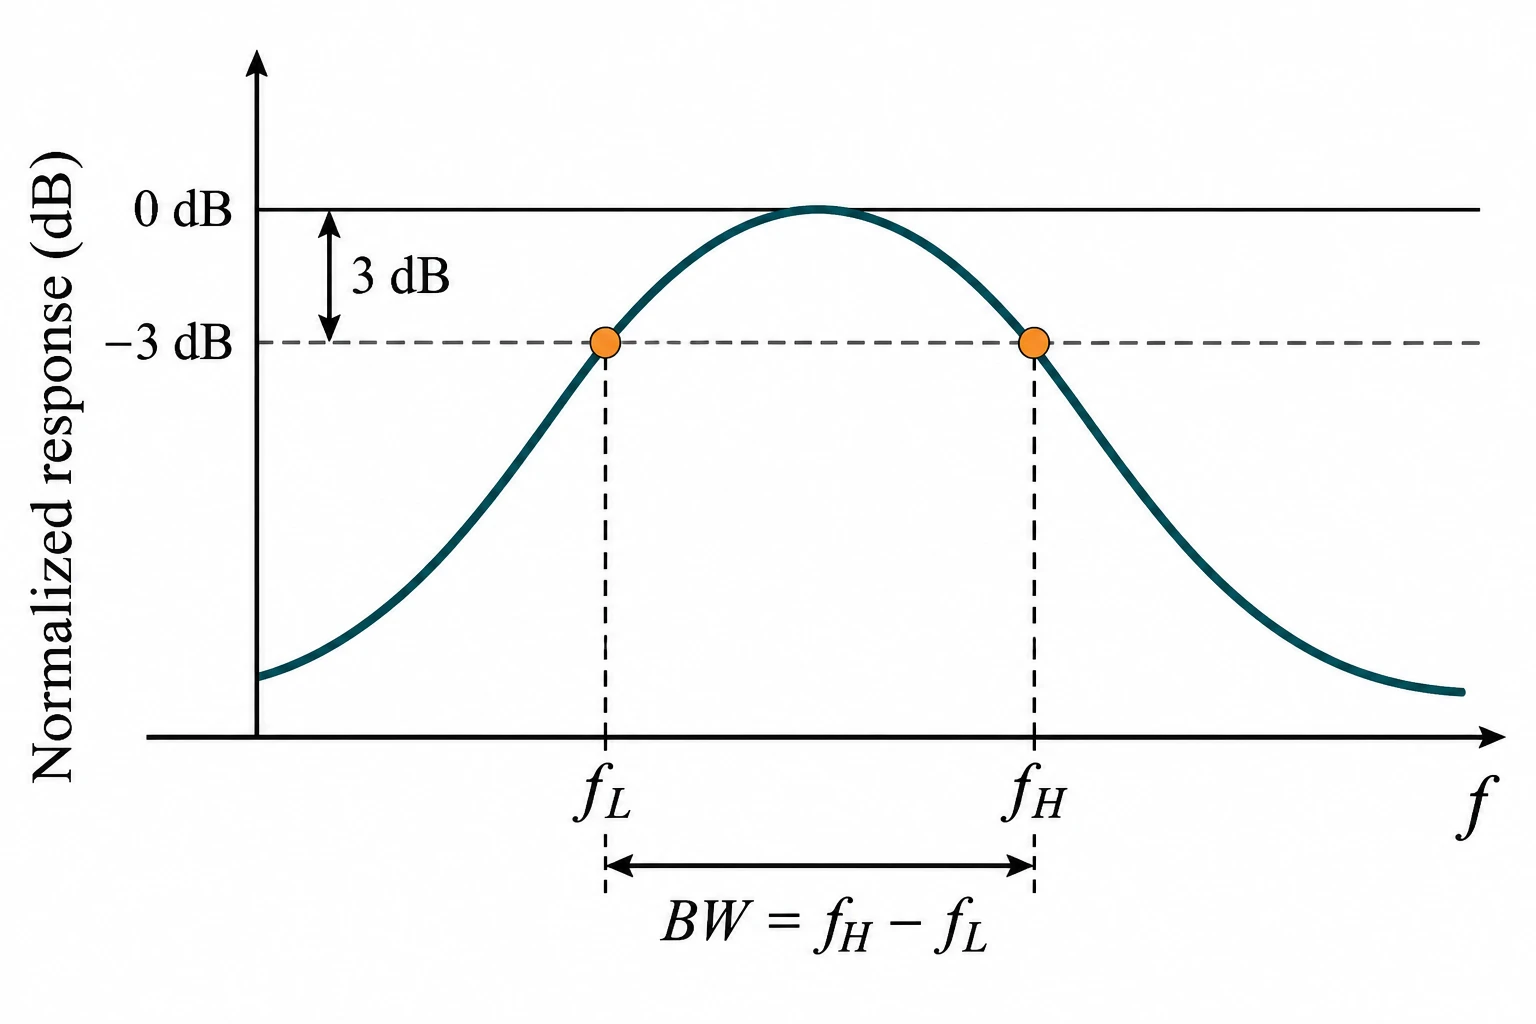
\includegraphics[width=0.85\linewidth]{figs/antena_response.png}
	\caption{پاسخ فرکانسی شماتیک آنتن؛ فرکانس‌های قطع پایین و بالا در سطح سه دسی‌بل کمتر از بیشینه و پهنای باند متناظر}
	\label{fig:antenna_frequency_response}
\end{figure}
توجه کنید که بازهٔ فرکانس کاری اعلام‌شده توسط سازنده یا فروشنده، لزوماً با معیار افت سه‌دسی‌بلی تعریف نشده است.

آنتن تهیه‌شده برای این آزمایش از صفحهٔ زیر خریداری شده است:
\begin{center}
	\href{https://www.javanelec.com/shop/product/13139/non-brand/antenna-gsm-3db-10cm/}{صفحهٔ آنتن در فروشگاه جوان الکترونیک}
\end{center}

به صفحهٔ محصول مراجعه کنید و بازه یا بازه‌های فرکانس کاری اعلام‌شده برای آنتن را در جدول زیر بنویسید. اگر چند بازهٔ مجزا ذکر شده است، هر بازه را در یک ردیف جداگانه ثبت کنید. اگر این اطلاعات در صفحه موجود نیست، عبارت «ذکر نشده است» را بنویسید.

\begin{table}[H]
	\centering\small
	\caption{بازه‌های فرکانس کاری آنتن بر اساس مشخصات صفحهٔ محصول}
	\label{tab:antenna_operating_frequency}
	\begin{tabularx}{\linewidth}{|c|X|X|}
		\hline
		\hdrrow \hdr{بازه} & \hdr{حد پایین بر حسب $\mathrm{MHz}$} & \hdr{حد بالا بر حسب $\mathrm{MHz}$} \\ \hline
		۱ & \rowstrut & \\ \hline
		۲ & \rowstrut & \\ \hline
		۳ & \rowstrut & \\ \hline
	\end{tabularx}
\end{table}


\زیرقسمت{ایده‌آل نظری در برابر اندازه‌گیری عملی}
\begin{table}[H]
	\centering\small
	\caption{فرض‌های تئوری و آنچه در اندازه‌گیری رخ می‌دهد}
	\label{tab:ideal8}
	\begin{tabularx}{\linewidth}{|r|X|X|}
		\hline
		\hdrrow \hdr{موضوع} & \hdr{مدل ایده‌آل} & \hdr{اندازه‌گیری عملی و پیامد آن} \\ \hline
		منبع نویز & $\mathrm{ENR}$ دقیقاً معلوم؛ حالت خاموش دقیقاً در $T_0$ & $\mathrm{ENR}$ عدم‌قطعیتی چند دهم دسی‌بل دارد و به فرکانس وابسته است؛ دمای اتاق $T_0$ نیست \\ \hline
		اتصال‌ها & بدون تلفات، منطبق & تلفات کابل و ناهماهنگی امپدانس، $\mathrm{ENR}$ مؤثر را تغییر می‌دهد \\ \hline
		گیرنده & خطی، با بهرهٔ ثابت & تراکم در حالت روشن یا تغییر بهره، $Y$ را کوچک و عدد نویز را بزرگ‌تر از واقع نشان می‌دهد \\ \hline
		خواندن توان & دقیق & نوسان آماری؛ با پهنای باند و زمان میانگین‌گیری کم می‌شود \\ \hline
		منبع دوتنی & دو تن خالص & خودِ منبع نیز محصول بین‌مدولاسیون می‌سازد؛ باید از سهم گیرنده جدا شود \\ \hline
		مدل غیرخطی & مرتبهٔ سوم بی‌حافظه & بریدگی مبدل، مرتبه‌های بالاتر؛ شیب سه همیشه برقرار نیست \\ \hline
	\end{tabularx}
\end{table}

%======================================================================
\isection{flow}{بلوک‌های \GR{} در این آزمایش}
%======================================================================
\begin{table}[H]
	\centering\small
	\caption{بلوک‌های اصلی (نام‌ها مطابق \GR{} \lr{3.10})}
	\label{tab:blocks8}
	\begin{tabularx}{\linewidth}{|l|X|}
		\hline
		\hdrrow \hdr{بلوک} & \hdr{نقش} \\ \hline
		\blk{Soapy RTLSDR Source} & گیرندهٔ تحت آزمون؛ بهرهٔ دستی، بهرهٔ خودکار خاموش \\ \hline
		\blk{Rotator} & تنظیم ریز فرکانس تا تن‌ها در جای اسمی خود بنشینند \\ \hline
		\blk{Frequency Xlating FIR Filter} & جدا کردن یک نوار باریک (برای هر تن) یا یک نوار پهنِ بدون سیگنال (برای نویز) \\ \hline
		\blk{RMS}، \blk{Log10}، \blk{QT GUI Number Sink} & توان هر نوار بر حسب \dBFS \\ \hline
		\blk{QT GUI Frequency Sink} & مشاهدهٔ طیف با میانگین‌گیری \\ \hline
	\end{tabularx}
\end{table}

%======================================================================
\isection{bulb}{مثال‌های محاسباتی}
%======================================================================
\begin{example}[رابطهٔ فریس]
تقویت‌کنندهٔ کم‌نویز
($G_1 = 15\un{dB}$، $\mathrm{NF}_1 = 1.5\un{dB}$)،
مخلوط‌کننده
($G_2 = -7\un{dB}$، $\mathrm{NF}_2 = 7\un{dB}$)
و تقویت‌کنندهٔ میانی
($\mathrm{NF}_3 = 5\un{dB}$).
به خطی:
$F_1 = 1.41$، $G_1 = 31.6$، $F_2 = 5.01$، $G_2 = 0.2$، $F_3 = 3.16$.
از رابطهٔ
\eqref{eq:friis}:
$F = 1.41 + 4.01/31.6 + 2.16/(31.6 \times 0.2) = 1.41 + 0.13 + 0.34 = 1.88$،
یعنی
\q{2.75}{dB}.
طبقهٔ سوم، با آن‌که آخر است، بیش از طبقهٔ دوم سهم دارد، چون تلفات مخلوط‌کننده بهرهٔ پیش از آن را کم کرده است.
\end{example}

\begin{example}[\lr{Y-Factor}]
با منبعی با
$\mathrm{ENR} = 15\un{dB}$
(نسبت خطی
$31.6$)
توان نویز در حالت خاموش
\q{-41.84}{\dBFS}
و در حالت روشن
\q{-32.78}{\dBFS}
خوانده می‌شود:
$Y = 9.06\un{dB}$
(خطی
$8.05$).
از رابطهٔ
\eqref{eq:yfactor}:
$F = 31.6/7.05 = 4.48$،
یعنی
$\mathrm{NF} = 6.5\un{dB}$.
(این اعداد از مدل گیرندهٔ تکلیف شبیه‌سازی در بهرهٔ ۴۰ دسی‌بل گرفته شده است.)
\end{example}

\begin{example}[آزمایش دوتنی و \lr{SFDR}]
دو تن هر کدام با توان
\q{-40}{dBm}
وارد می‌شوند و محصول مرتبهٔ سوم
\q{50}{dB}
پایین‌تر از هر تن دیده می‌شود:
$\mathrm{IIP3} = -40 + 25 = -15\un{dBm}$
و، اگر مدل مرتبهٔ سوم برقرار باشد،
$P_{\mathrm{1dB}} \approx -24.6\un{dBm}$.
با
$\mathrm{NF} = 6.5\un{dB}$
و پهنای باند
\q{10}{kHz}،
کف نویز
$-174 + 6.5 + 40 = -127.5\un{dBm}$
و
$\mathrm{SFDR} = \tfrac{2}{3}(-15 + 127.5) = 75\un{dB}$
است.
\end{example}

%======================================================================
\isection{pencil}{تکالیف گزارش پیش‌از‌جلسه}
%======================================================================
شش جزء الزامی آیین‌نامه (بند
\bnd{۳-۱})
برای این آزمایش:

\begin{task}{خلاصهٔ یک‌صفحه‌ای}[مطالعهٔ منبع]
منبع‌های تعیین‌شده را بخوانید و در حداکثر یک صفحه بنویسید: عدد نویز چه چیزی را می‌سنجد، روش
\lr{Y-Factor}
چرا به اندازه‌گیری مطلق توان نیاز ندارد، و نقطهٔ تقاطع مرتبهٔ سوم چه چیزی را پیش‌بینی می‌کند.
\end{task}



\begin{task}{شبیه‌سازی آفلاین}[کار با مدل گیرنده]
فلوگراف آمادهٔ
\code{lab02_sim.grc}
را از مدرس بگیرید. این فلوگراف یک گیرندهٔ مدل را شبیه‌سازی می‌کند (طبقهٔ ورودی با عدد نویز و غیرخطی‌بودن مرتبهٔ سوم، بهرهٔ قابل تنظیم و مبدل هشت‌بیتی، این مدل در شکل ~\ref{fig:simulator} نشان داده شده است.) و همان اندازه‌گیرهایی را دارد که در جلسه به کار می‌برید. با آن:
\begin{enumerate}
\item در بهرهٔ ۴۰ و سپس ۱۰ دسی‌بل، عدد نویز را با روش
\lr{Y-Factor}
اندازه بگیرید. برای هر بهره
$\mathrm{ENR}$
مناسبی برگزینید و دلیل انتخاب را بنویسید.
\item در بهرهٔ ۴۰ و سپس صفر، با جاروب توان تک‌تن (گام یک دسی‌بل نزدیک تراکم) منحنی خروجی بر حسب ورودی را رسم و
$P_{\mathrm{1dB}}$
ورودی را بخوانید.
\item در بهرهٔ صفر آزمایش دوتنی را در چند سطح انجام دهید: شیب محصولات مرتبهٔ سوم را بسنجید،
$\mathrm{IIP3}$
را استخراج و با
$P_{\mathrm{1dB}} + 9.6\un{dB}$
مقایسه کنید.
\item همان آزمایش دوتنی را در بهرهٔ ۴۰ تکرار کنید. محصولات بین‌مدولاسیون چگونه پدیدار می‌شوند و چرا این‌جا نقطهٔ تقاطع معنای روشنی ندارد؟
\item عدد نویز و
$P_{\mathrm{1dB}}$
را برای بهره‌های صفر تا ۵۰ (با گام ۱۰) در یک جدول بنویسید و بهره‌ای را بیابید که فاصلهٔ
$P_{\mathrm{1dB}}$
تا کف نویزِ نوار
\q{10}{kHz}
در آن بیشترین است.
\end{enumerate}
\end{task}

\begin{figure}[htbp]
    \centering
    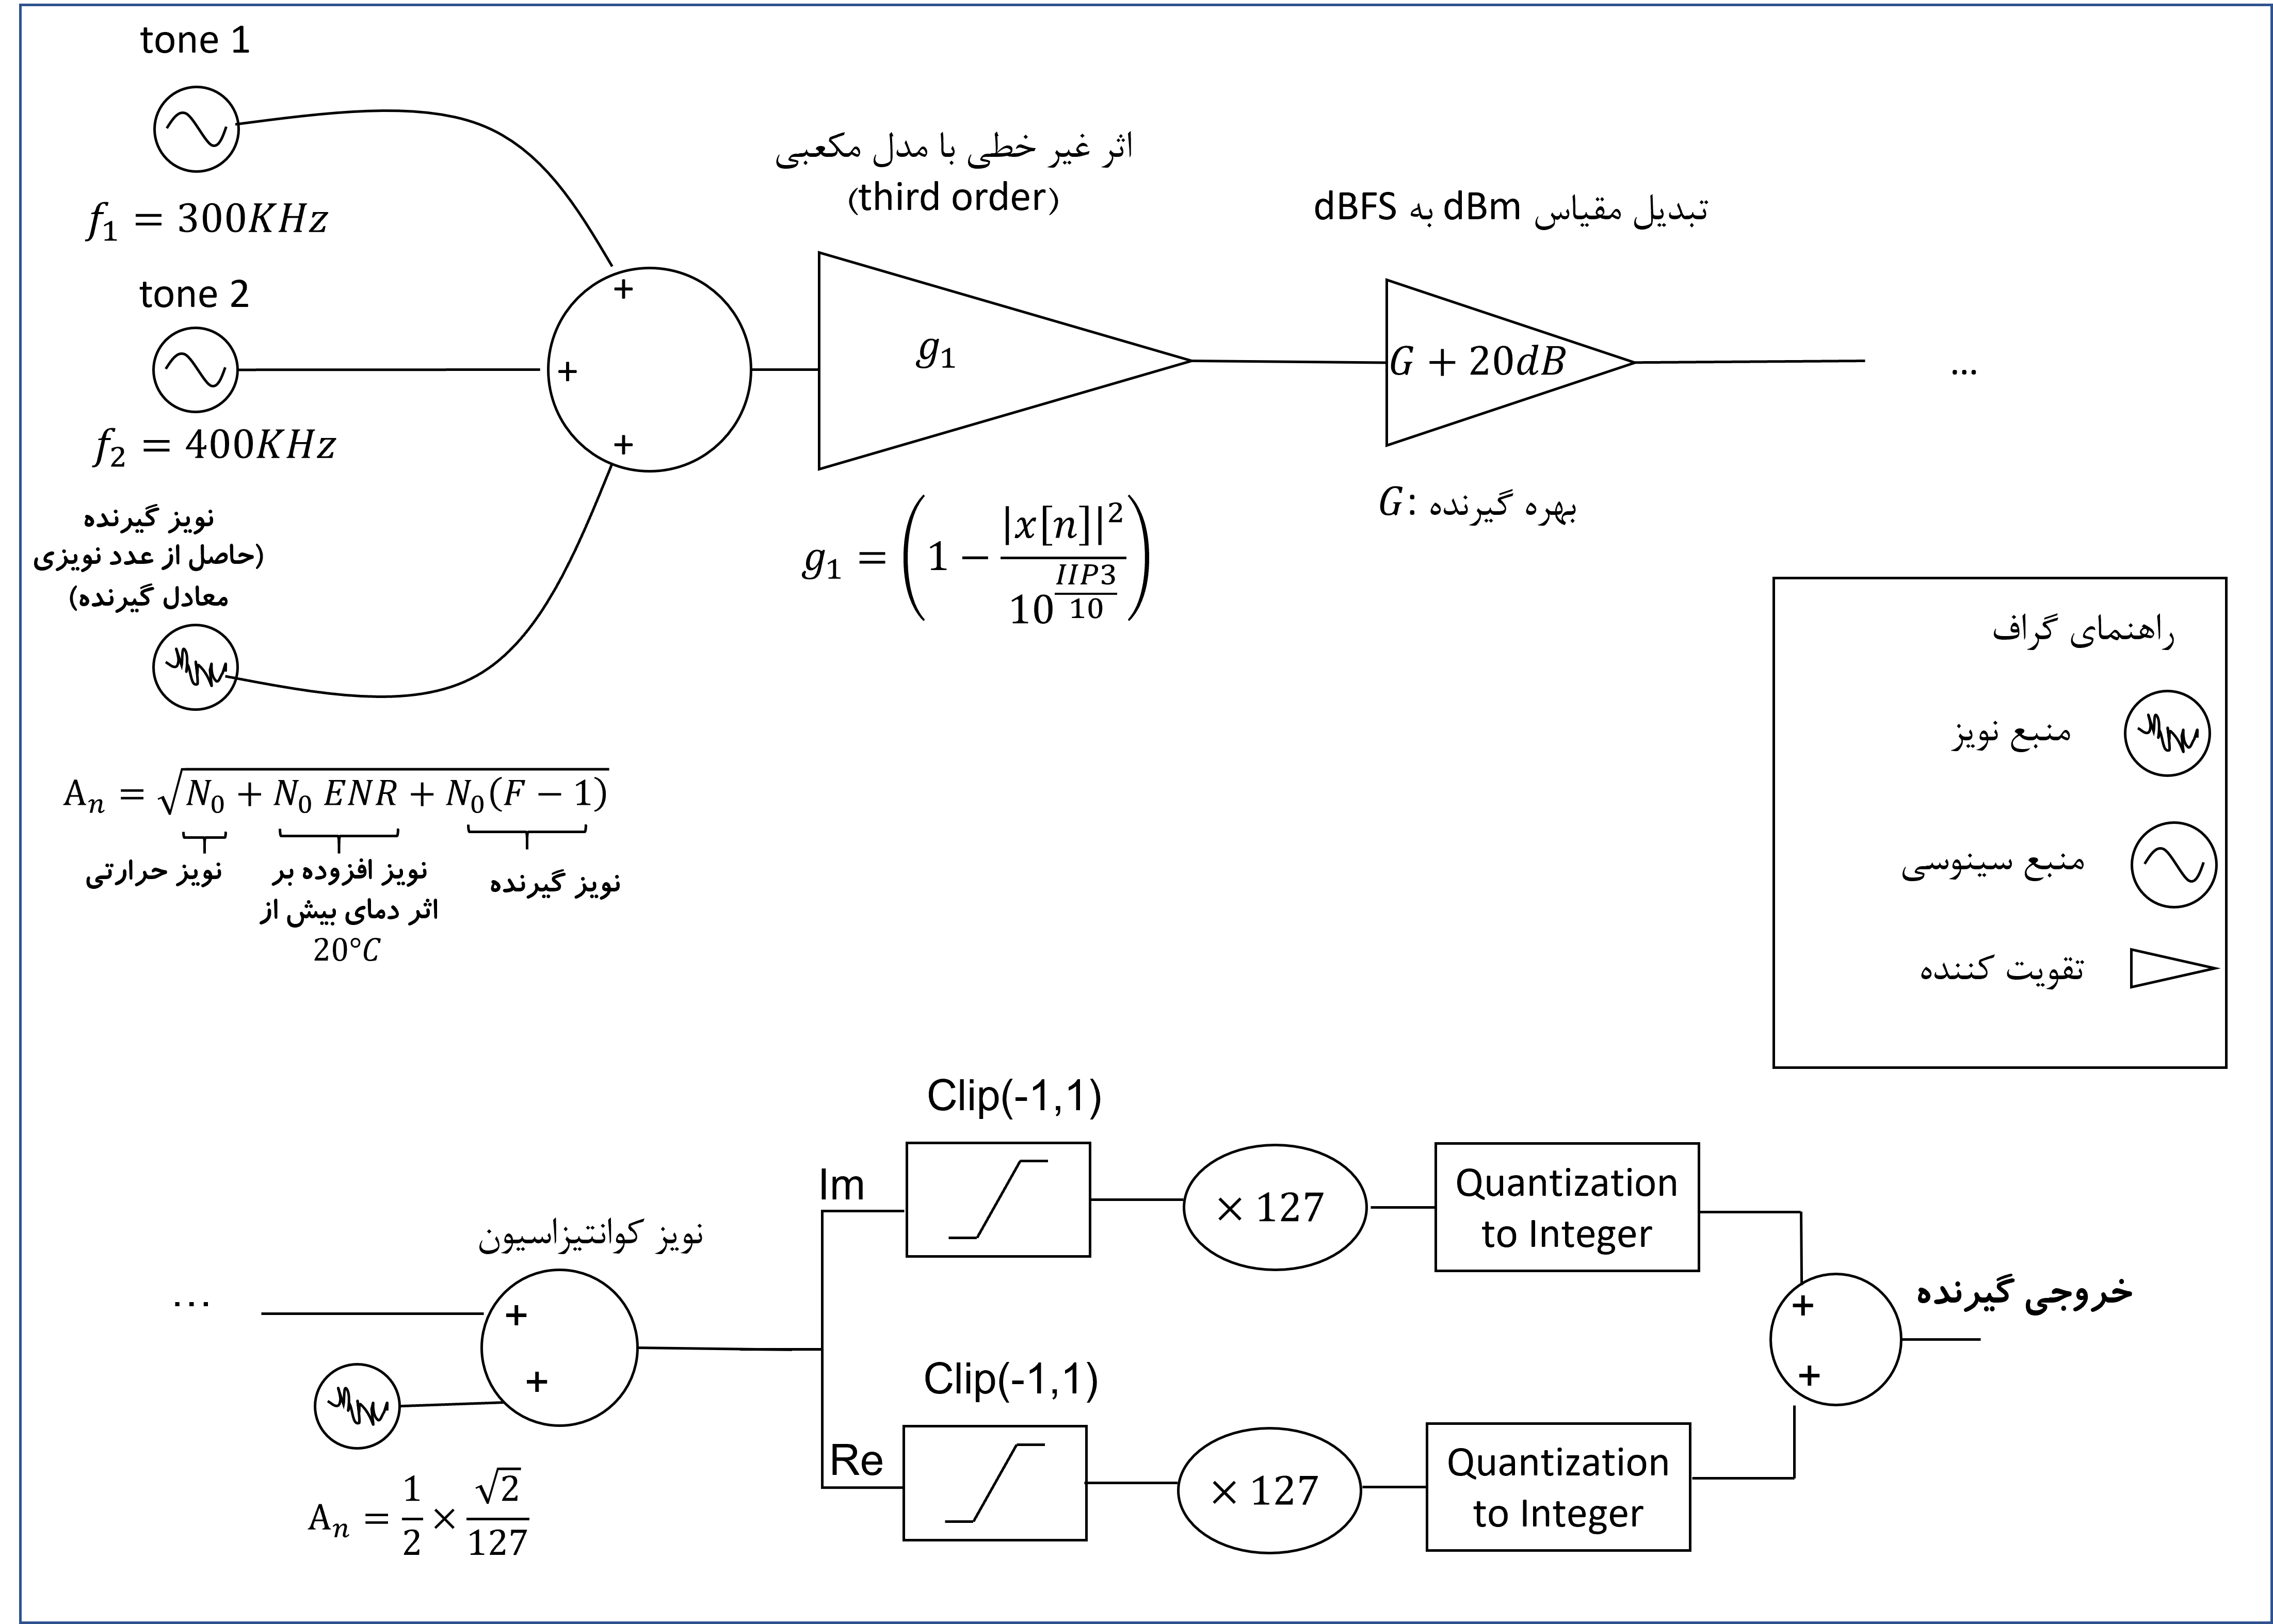
\includegraphics[width=\textwidth]{figs/Simulator_Diagram.png}
    \caption{بلوک دیاگرام مدل گیرنده SDR}
    \label{fig:simulator}
\end{figure}

%======================================================================
\isection{warn}{پیش از ورود به آزمایشگاه بدانید}
%======================================================================
\begin{safetybox}[سطح ورودی گیرنده (آیین‌نامه، بند \bnd{۸-۱})]
\begin{itemize}
\item توان ورودی گیرنده هرگز از
\q{-10}{dBm}
بیشتر نشود. پیش از اتصال هر منبع، سطح خروجی آن را حساب کنید و در صورت نیاز تضعیف‌گر بگذارید.
\item خروجی سیگنال ژنراتور را پیش از بستن یا بازکردن کابل خاموش کنید و جاروب توان را همیشه از پایین‌ترین سطح آغاز کنید.
\item منبع نویز و ورودی گیرنده به تخلیهٔ الکتریسیتهٔ ساکن حساس‌اند؛ پیش از دست‌زدن به اتصال‌ها بدنهٔ دستگاه را لمس کنید و اتصال‌ها را با دست و بدون فشار ببندید.
\item اگر به‌جای ژنراتور از فرستندهٔ
\lr{SDR}
استفاده می‌کنید، تضعیف‌گر
\q{30}{dB}
الزامی است.
\end{itemize}
\end{safetybox}

%======================================================================
\isection{list}{چک‌لیست آمادگی}
%======================================================================
\begin{checklist}
\item گزارش پیش‌از‌جلسه
(\lr{PDF}
و
\lr{HTML})
بارگذاری شده است.
\item فلوگراف
\code{lab02_meas.grc}
را از روی دستور کار از پیش ساخته‌اید (اندازه‌گیرها را می‌توانید از فلوگراف مدل بردارید).
\item جدول طراحی و جدول پیش‌بینی کامل است و هر عضو می‌تواند از دو عدد
\dBFS{}
عدد نویز را حساب کند.
\end{checklist}

%======================================================================
\isection{book}{مراجع}
%======================================================================
\begin{latin}\small
\begin{enumerate}[label={[\arabic*]},leftmargin=2.2em,itemsep=1pt]
\item D. M. Pozar, \textit{Microwave Engineering}, 4th ed. Hoboken, NJ: Wiley, 2012.
\item Keysight Technologies, ``Noise figure measurement accuracy: the Y-factor method,'' Application Note.
\item B. Razavi, \textit{RF Microelectronics}, 2nd ed. Upper Saddle River, NJ: Prentice Hall, 2012.
\item GNU Radio project, GNU Radio Wiki: block documentation. [Online]. Available: https://wiki.gnuradio.org
\end{enumerate}
\end{latin}

\end{document}
